\chapter{基于web可视化工具概述}
\chaptermark{基于web可视化工具概述}
	%GBrowse
	\section{GBrowse}
		\subsection{概述}
		GBrowse是基因组浏览器(GenomeBrowse)的缩写。它是一种基于WEB服务的应用程序,用来可视化基因组的注释及基因性态等其他信息。GBrowse拥有通用模式的便捷和自定义模式的灵活性,用户可以通过网页浏览基因组可视化信息,可以通过搜索功能查找特定基因组,对于查看区域的基因组可以通过缩放进行更加有效的查看,同时提供对基因组相应序列数据的下载,支持gff3,fasta等格式的数据下载。现在GBrowse已经有多个版本,GBrowse1.X版本在2002年就已经开始使用,经过将近十年的发展,各方面都较为成熟,性能比较稳定。GBrowse2.0版本在原有的版本上进行了重写,使用了AJAX技术可以进行动态更新,拥有更好的用户体验,同时对于服务端的性能有了部分的提升。同时GBrowse作为基于web服务的浏览器不用安装,无需进行繁琐的软件配置,用户只需要通过网页浏览器连接到 Internet 就可以使用,对用户个人PC 的要求不高,而且由于数据存储在服务器端,所以用户本地电脑不用消耗太多存储空间来贮放数据。
		\subsection{可视化方式}
		GBrowse用 track的方式进行可视化相关基因组信息,通过对track进行缩放进行细化展示基因跨度可以展示基因组整体效果。GBrowse附带了一个大型字形库,包括饼图,点图,直方图和适用于定量数据的XY图,以及描述序列和序列注释的预期字形数组。通过合理地配置及编码可以实现基因组基因的可视化。
		\subsection{可视化内容}
		GBrowse可视化内容由可视化图谱进行具体显示,可视化图谱可以分为三个部分:overview(概述),region(区域),details(细节)。
		\begin{itemize}
			\item  overview(概述)显示基因组背景,通常是整个组装的染色体或序列组合的大部分,例如支架或重叠群。
			\item region(区域)显示感兴趣区域周围的一部分基因组。
			\item details(细节)显示与概览选择矩形相对应的基因组的放大视图。细节区域包含一个或多个轨迹,显示已经放置在基因组上的注释和其他特征。详细视图由从显示器的一端水平延伸到另一端的多个不同的轨迹组成。每个轨道对应于不同类型的基因组特征,并且通过独特的图形形状和颜色来区分。如图一所示,可以明确地看到。
		\end{itemize}
	GBrowse从版本2.0开始,通过提供直接显示SAM和BAM序列对齐文件,GBrowse支持下一代排序(NGS)数据。SAM/BAM轨道提供语义缩放,并支持本地和远程数据源。可以上传的格式有GFF3,SAM/BAM等多种数据格式的文件。
		\begin{figure}
			\centering
			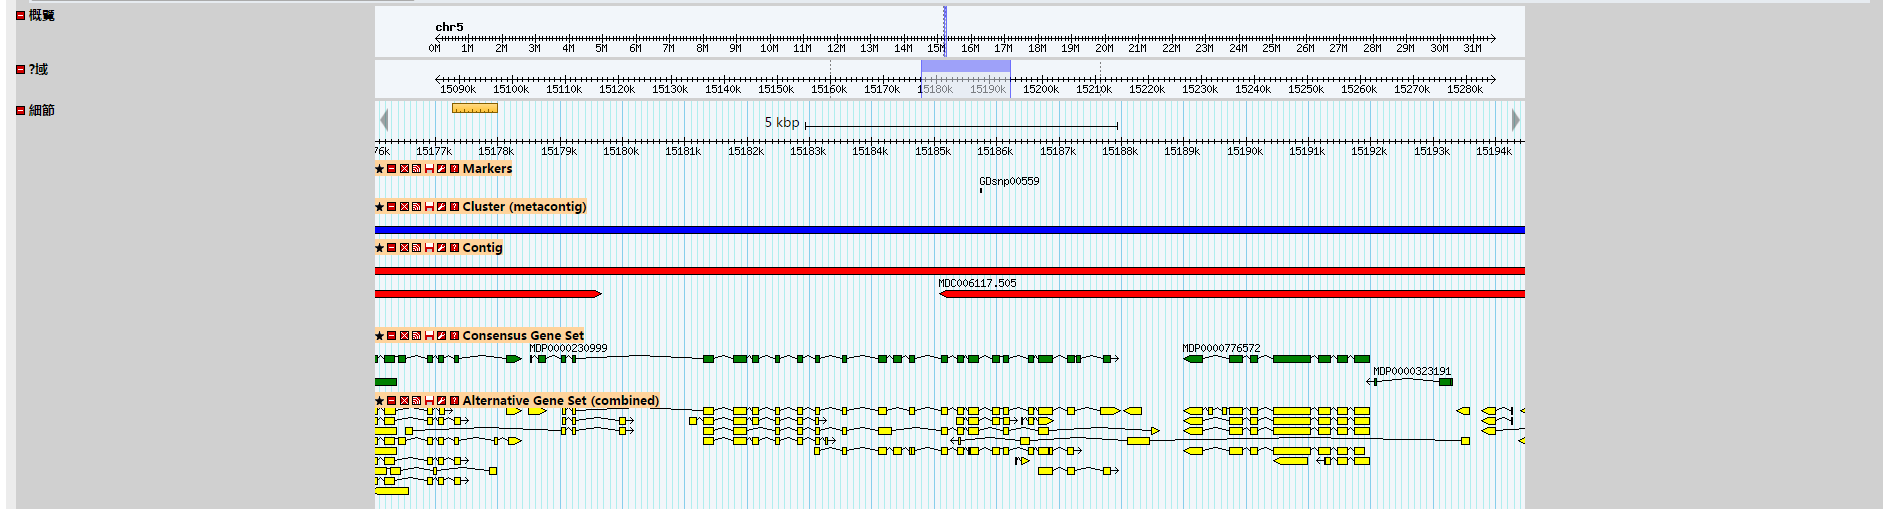
\includegraphics[width = .9\textwidth]{2-1.png}
			\caption{GBrowse页面内容展示图}
		\end{figure}	
		\subsection{系统架构}
		GBrowse是一个Web应用程序,可分为Web服务器端和Web浏览器客户端。GBrowse的服务器端是用Perl编写,部分核心工能由C代码来实现,以达到高性能的需求。服务器端管理一系列包含基因组注释信息的数据库,从Web浏览器接收用户对感兴趣可视化基因区域的请求,并将这些区域显示为PNG,SVG或PDF图像等高清图像返回给Web浏览器端。在Web浏览器端,一系列由Javascript编写的功能函数处理用户界面,实现了跨基因组平移和缩放,通过点击拖动选择一个区域,通过弹出菜单配置曲目并上传曲目数据。\\
		\indent GBrowse的组成可以分成多个部分;顶层是由GBrowse中的CGI模块构成,用来与web服务器进行交互,通过接收用户的相关操作信息,将反馈相关数据给web服务器,在由web服务器将数据返回到用户浏览器,完成用户与服务器之间的交互,同时GBrowse接受第三方扩展,方便对其进行功能扩展。中间层是有PERL库中Bio::Graphics模块与PerlBio模块组成,中间层是GBrowse的核心层,其实现了数据库和用户接口的交互,它将数据库与用户接口进行分离,抽象了数据库连接模块,避免了不同数据库下数据格式存在差异性及连接不兼容的细节问题,从而使得从不同的数据库中读取数据后采用相同数据格式进行显示而且支持多种数据的使用。该模块可以存储jpeg、wbmp、png等不同格式图片并将其转换统一显示到浏览器端。底层是由GBrowse可以使用的数据库类型组成,目前支持MySQL,SQLite,BerkeleyDB等数据库,这种设计可以让GBrowse对大多数主流数据库支持良好,设计者只需编写一个相应的数据库适配器,便可通过该程序将数据导入库模块。\\
		\indent GBrowse支持广泛的基因组数据库和视图是GBrowse最灵活的功能之一。一系列数据适配器扩展允许GBrowse将数据加载到内存,同时支持大型SQL和NoSQL数据库文件及远程数据源和专门的文件格式(如BAM对齐文件)。基因组特征可以由大量可重复使用的“字形”(即feature大致为75个)代表,其范围从通用有色盒子到SNP单倍型区段之间的连锁不平衡的高度特异性表示。
		\begin{figure}[!ht]
			\centering
			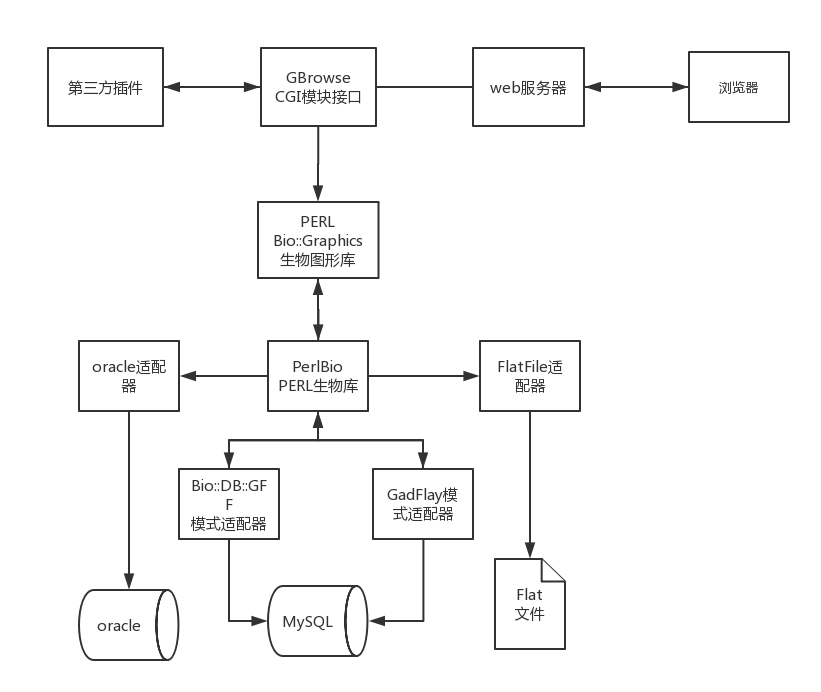
\includegraphics[width = .6\textwidth]{2-2.png}
			\caption{GBrowse系统结构}
		\end{figure}
		\subsection{运行机理}
		当用户向GBrowse发出浏览数据请求时,浏览器根据URL或者AJAX向服务器发送用户请求,服务器接收到用户请求,判断是不是一个静态文件请求,若不是则判断是不是一个CGI可执行文件请求,若是将请求交给GBrowse的CGI扩展,并执行相应的Perl脚本,执行完脚本GBrowse的CGI模块将产生的数据返回给Web服务器,Web服务器接收到数据后再将数据返回给浏览器,触发浏览器端的脚本文件执行使浏览器重新渲染Web页面产生可视化效果。如图2-3GBrowse的CGI模块请求处理流程。
			\begin{figure}[!ht]
				\centering
				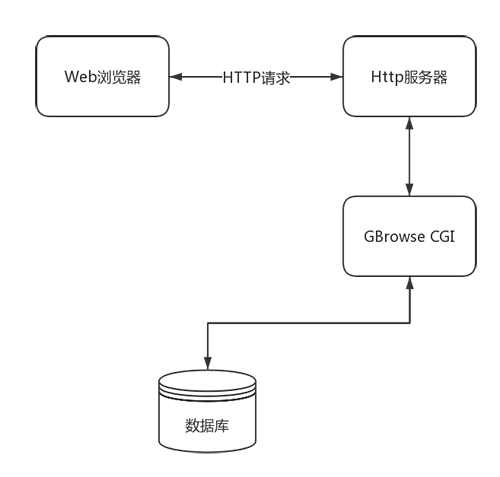
\includegraphics[width = .5\textwidth]{2-3.png}
				\caption{GBrowse模块请求处理}
			\end{figure}
		\subsection{优缺点}
		优点:GBrowse支持大部分基因组数据集格式,对于浏览器的兼容性良好,可以友好的显示在web端,并且拥有良好的跨平台性和兼容性;GBrowse可视化方式多种多样,支持用户上传数据,支持用户管理功能。\\
		\indent 缺点:GBrowse需要许多第三方库。特别是,为了显示NGS测序数据,GBrowse需要Samtools和BigWig库。由于这些依赖关系的安装对于初次安装者来说可能是迷茫且令人困惑的,容易使安装者无法准确地定位出错信息,无法很好地解决环境安装和依赖管理的问题。同时GBrowse2.0作为新开源的基因组可视化工具,存在着部分问题,不适宜新手进行安装使用。针对性能和用户体验方面,GBrowse的大部分工作依赖于服务器端地处理,对服务器端地性能要求过高;用户在通过GBrowse进行基因可视化对比查看时,当需要放大缩小即进行其它操作时,GBrowse会向服务端进行请求,延长用户等待时间,具有较差的用户体验。
		%JBrowse
	\section{JBrowse}
		\subsection{概述}
		JBrowse是一个开源的便携式的基于JavaScript的基因组浏览器,并以GBrowse继任者为目标。它运行速度非常快并且支持大型数据集。JBrowse完全由JavaScript和HTML5构建的,几乎所有的工作,发生在用户的Web浏览器端,对服务器有最低的要求。事实上,JBrowse没有后端服务器代码,后端只是用于格式化数据文件并通过HTTP请求将数据传输到浏览器端。JBrowse可以快速,平滑滚动和缩放,支持缩放多基因组和基因组的深度覆盖测序。 JBrowse具有高度的可扩展插件架构,可以很方便地嵌入任何Web应用中。JBrowse具有良好的跨平台性,目前JBrowse在Electron跨平台应用开发框架下逐步推出Windows等操作系统下的应用软件,方便用户可视化数据。
		\subsection{可视化方式}
		JBrowse用 track 的方式进行可视化,提供平滑的动态移动和缩放功能,也有导航和通道的选择。JBrowse可以展示多种 track 视图,除基本视图外,还可以显示非翻译区、外显子、内含子结构等。
		
		\subsection{可视化内容}
		JBrowse可以展示基因组整体视图,也可以细化展示基因跨度、tRNA、转座子、寡核苷酸、蛋白质结合位点、增强子、基因调控区域、非编码RNA、点突变、序列变异信息等其它基因信息。用户可以自己上传需要可视化的内容的相关基因数据,支持GFF、GFF3、WIG、BED、FASTA、Wiggle、BigWig、BAM 等多种格式的数据文件。如图2-5所示
		\begin{figure}[!ht]
			\centering
			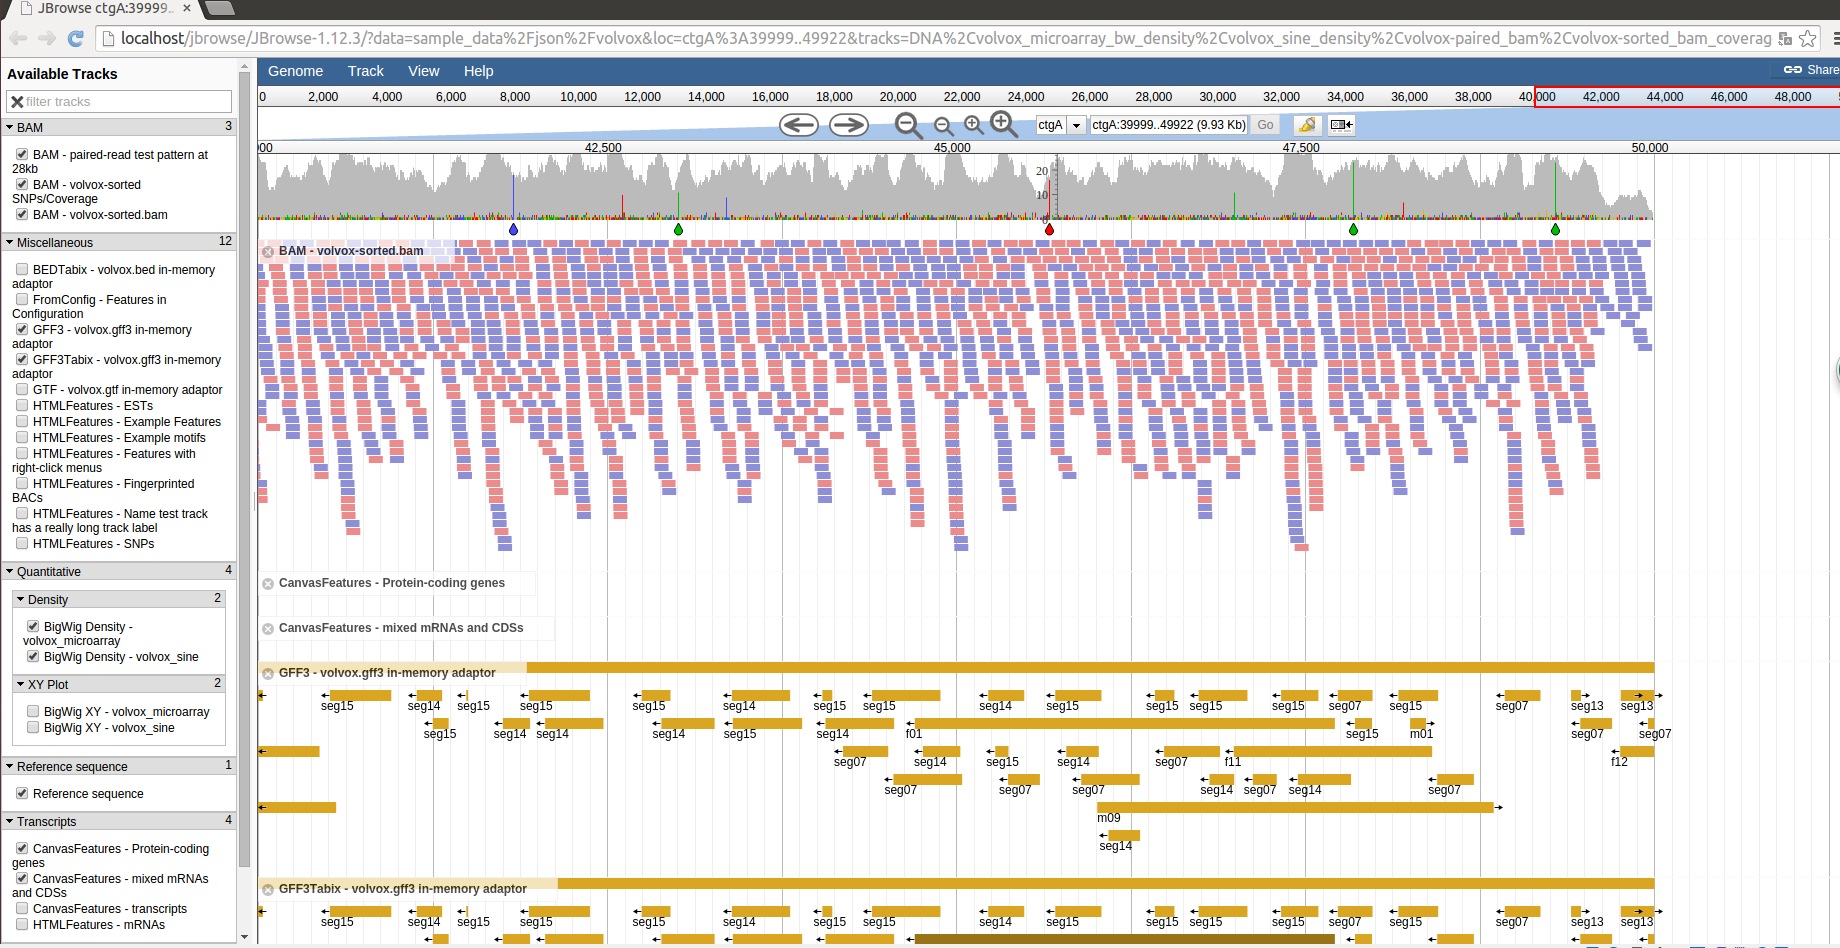
\includegraphics[width = .6\textwidth]{2-4.png}
			\caption{JBrowse可视化内容}
		\end{figure}
		\subsection{系统架构}
		JBrowse 完全由Javascript和 HTML5构建实现,对外提供 Javascript API功能接口,后端数据通过Perl工具进行处理。Web端对浏览器的要求是需要支持 HTML5 中的新标签(如 Canvas),目前主流的浏览器支持良好。后台服务器端主要采用 Json文件进行数据存储,  Json作为一种轻量级的数据交换格式,是基于Javascript语言规范进行设计,属于 Javascript的一个子集,在Javascript中的以对象和数组的形式存在,因此可以实现较快的前后台通信,提高通信速度加强用户体验。\\
		\indent JBrowse分为前端和后端,如图2-5所示。在后端JBrowse可以分为三部分,数据库适配器,配置文件,数据管理工具;JBrowse数据适配器由Perl编写实现,有易扩展的特性;JBrowse对多种数据适配器支持,比如Bio::DB::SeqFeature::Store,数据适配器的多样使JBrowse支持多种数据类型。数据处理工具进行预处理,将数据的功能曲目存储到嵌套的列表NCL中,并将基因名称和其他文本信息存储到Patricia中,将Wiggle数据进行预渲染成图片存储到服务器端,预处理的过程中将会对数据进行压缩处理,对于预处理数据是不可避免的,对于JBrowse来说大部分图像渲染依赖客户端,客户端的性能过分依赖于用户的硬件及Web浏览器,所以服务端的数据预处理尤为重要。通过制定相应的配置文件可以管理JBrowse的功能,也可以更加人性化定制数据可视化显示后的效果。\\
		\indent 在客户端可以根据显示的内容进行划分,序列轨迹,特征轨迹,图像轨迹,Javascript通过解析服务端查询服务端通过HTTP请求发送过来的tile索引文件并检索和组织图片进行显示,并且可以将渲染的图片扩展到任意维度。JBrowse通过使用Html及Canvas来显示图形内容。
		\begin{figure}[!ht]
			\centering
			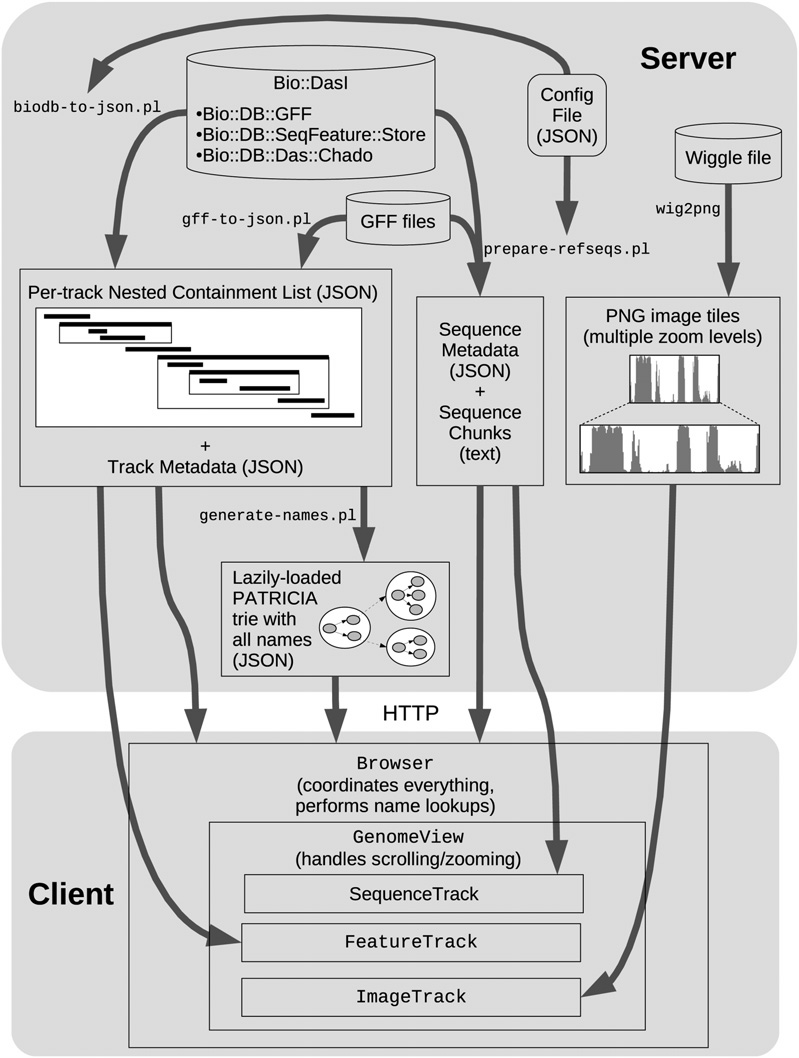
\includegraphics[width = .4\textwidth]{2-5.png}
			\caption{JBrowse系统架构}
		\end{figure}
		\subsection{运行机理}
		JBrowse的工作流分为服务端工作流和前端工作流。当用户通过浏览器对目标网址进行访问时服务端将预处理后的数据进行以Json的形式进行传送到前端,前端通过Javascript引擎进行加载处理,并渲染生成基因数据图像。\\
		\indent 服务端将对于后端工作流大致可以概括为基本调用,汇编,注释,对齐和比较注释,并生成了JBrowse文件。服务端将序列文件进行注释,对比注释,phastCons等操作对数据进一步进行数据整理和压缩,通过HTTP请求进行数具传输。
		\begin{figure}[!ht]
			\centering
			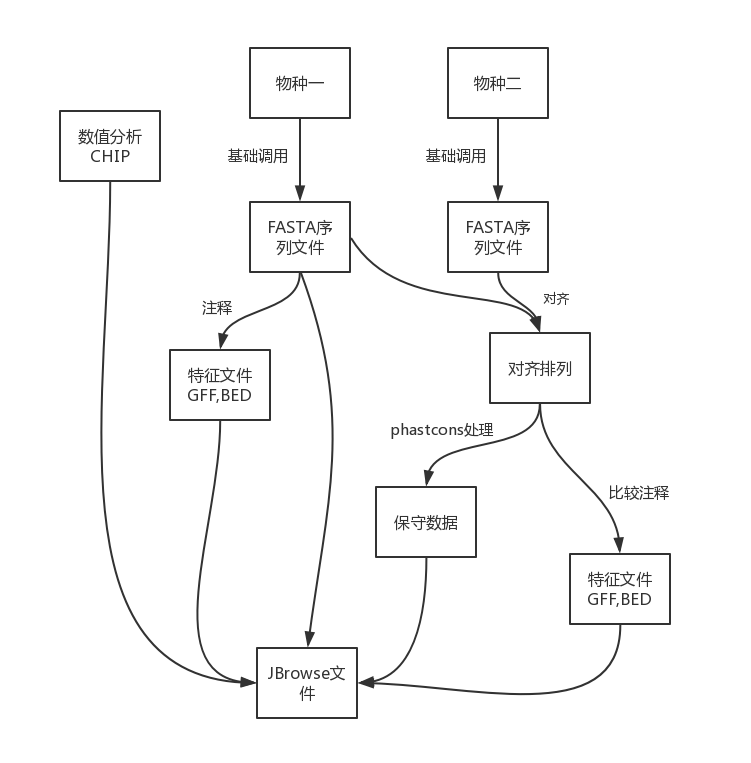
\includegraphics[width = .4\textwidth]{2-6.png}
			\caption{JBrowse工作流图}
		\end{figure}
		\subsection{优缺点}
		优点:JBrowse 属于新一代基因组浏览器,作为GBrowse的继任者,是基于最新的前端技术开发的。在 JBrowse 中,服务器端的负荷极大地降低,后台服务器只需要向浏览器客户端发送数据文件,将繁杂的计算工作从服务端脱离出来,大量计算工作被合理分配到了前端。同时,JBrowse对Cookies技术也得到了很好的支持,可以有效记录用户的喜好。\\
		\indent 缺点: JBrowse 把可视化主要工作放在了浏览器端,但其可视化方法仅是一些普通的HTML 标签实现,造成可视化不友好等问题。同时浏览器在绘制图像时需要运行大量的JavaScript代码,而且目前主流浏览器对 HTML5 中新标签的支持不完善,造成用户体验不佳等问题。
	\section{UCSC Genome Browser}		
			\subsection{概述}	
			UCSC Genome Browser是由University of California Santa Cruz (UCSC) 创立和维护的,该站点包含有人类、小鼠和大鼠等多个物种的基因组草图,并提供一系列的网页分析工具。站点用户可以通过它可靠和迅速地浏览基因组的任何一部分,并且同时可以得到与该部分有关的基因组注释信息,如已知基因,预测基因,表达序列标签,信使RNA,CpG岛,克隆组装间隙和重叠,染色体带型,小鼠同源性等。用户也可以因为教育或科研目的加上他们自己的注释信息。UCSC Genome Browser目前应用相当广泛,比如Ensembl 就是使用它的人类基因组序列草图为基础的。
			\subsection{可视化方式}		
			UCSC Genome Browser 以 track(轨道)的方式来展示相关信息。 Track 表现为横向或纵向的条带,条带上不同区域分别用不同的颜色、线、方块等表示不同的生物含义,因形状类似于赛场的跑道,故翻译为轨道,如图 1 中红色矩形条状框内即为一条轨道。系统主界面从上到下可分为三块:检索查询、可视化(图 1)和轨道管理. a.检索查询,包括直接通过染色体区域范围查询、根据基因名称进行查询、对页面中现有范围的左右平移和倍数缩放等;b.可视化展示,每条样本数据都用一条轨道来表示,并且目前提供5种展示示模式(hide、dense、squish、pack、full);c.轨道数据管理,主要包括 track 的分组管理、展示模式的管理以及用户自己上传数据的可视化等。研究者可以通过控制图片下方的下拉菜单来选择展示哪些 track。 每个track 名字都链接到一个特定的网页,从中可以查看该 track 数据的计算方式,还可能有相应的文献或者序列信息等。页面中不同的元素代表不同的含义,比如在基因结构视图中,盒形代表外显子,线形代表内含子。 研究者可以点击 Genome Browser上相应按钮获得更多注释信息, 像正向 选择(positive selection)基因等。
			\subsection{可视化内容}		
			UCSC基因组浏览器提供了多样化的注释数据集(称为“轨迹”并以图形方式呈现),包括mRNA比对,DNA重复元件的映射,基因预测,基因表达数据,疾病关联数据(代表基因的关系疾病)和市售基因芯片(例如Illumina和Agilent)的映射。显示的基本范例是在水平维度上显示基因组序列,并显示mRNA的位置,基因预测等的图形表示。沿着坐标轴的颜色块显示各种数据类型对齐的位置。在单个坐标轴上显示这种大量数据类型的能力使浏览器成为数据垂直整合的便利工具。\\
			\indent UCSC浏览器与其他基因组浏览器区分开来的一个独特而有用的功能是显示器的不断变化的性质。可以显示任何大小的序列,从单个DNA碱基到整个染色体(人类chr1 = 2.45亿碱基,Mb)和完整的注释轨迹。研究人员可以显示单个基因,单个外显子或整个染色体带,显示数十个或数百个基因以及许多注释的任意组合。方便的拖放功能允许用户选择基因组图像中的任何区域,并将其扩展到占据全屏。
			\subsection{系统架构}		
			UCSC Genome Browser 的开发,起源于一小段应用于 C. elegans 基因预测拼接图谱的 C 语言脚本,后期通过不断扩充,才变成现在这样强大的一个分析工具。 现在 UCSC 的主要开发语言是Java/Python,后台数据库依赖于 mysql,而且提供mysql 的公共接口,只要用户本地电脑装有 mysql客户端,就可以通过 UCSC 提供的接口访问网站后台的数据库;对于前台要求,UCSC 可以较好地兼容 IE、Chrome、Firefox 等主流网络浏览器。UCSC 是完全开源的,用户可以下载到完整源码。
			\subsection{优缺点}
			优点:	UCSC Genome Browser 是一个非常综合的基因组浏览器,包含物种数比较多,可视化内容也比较齐全。
			\indent 缺点:从 web 技术的发展历程,可以将其分为几个阶段:web1.0 时代用户被动接收网站单向发布的信息,以个人网站为代表;web2.0 时代的特征则是开放、去中心化,用户参与信息发布和分享,以博客为代表;新一代 web 技术是对 HTML5 及其周边相关应用开发的统称,它可以支持更多的人机互动,并能实现很大程度的智能化。局部刷新技术是
			指,当网页中的某一个元素或标签需要改变时,不重新加载整个页面,而只对需要改变的部分进行刷新的技术。然而遗憾的是,UCSC Genome Browser的开发年代尚处在 web1.0 时代,没有充分应用新一代 web 技术和局部刷新技术,所以 UCSC 中部分程序驱动的脚本对用户访问频率有一定限制:以BLAT 脚本为例,它最多支持每 15 s 一次用户点击加载,一天最多只能支持 5000 次后台加载。